% !TeX spellcheck = en_GB

\chapter{Introduction}
\label{ch:introduction}
\lhead{Chapter \thechapter. \emph{Introduction}}

\section{\acrfullpl{manet}}\label{manets}

With the explosive growth in the use of mobile telephony and the increasing miniaturisation and efficiency gains of portable communications devices, the classical paradigm of a broadcast/receiver (or server/client) has given way to an increasing use of decentralised, ad-hoc networks that take advantage of this network dynamism to improve service efficiency.

Whether these networks are decentralised cellular / \gls{rf} / 802.11 WiFi networks for use in disaster relief areas \cite{Milliken2015} or biologically inspired wireless sensor networks for low-energy, low-maintenance environmental monitoring \cite{Nicholson2008,Selvakennedy2007}, \gls{manet} theory developed over the past 30 years has gone from it's first formal definition, emerging from \glspl{darpa} Packet Radio Network research \cite{Jubin1987}, to being an integral part of modern practical communications.

Minimally, a \gls{manet} consists of of a collection of mobile physical entities (nodes) that communicate cooperatively to collect, distribute, disseminate, and collate data and/or influence across an area.
In most cases \gls{manet} nodes incorporate bi-directional transceivers to send and receive data\footnote{However this bi-directionality is not always a requirement; for example in the area of \gls{wsn} \cite{Akyildiz2002})}
\glspl{manet} may utilise omnidirectional, static, or steerable communications antennae, and a selection of protocols such as WiFi, Bluetooth, \gls{gsm}, \gls{umts}, Optical or Acoustic, and may incorporate a range of mobilities across nodes, from static devices, terrestrial and marine surface platforms, as well as aerial and underwater platforms.
A core characteristic of \glspl{manet} is the inclusion and integration of heterogeneous node collections, i.e.\ different nodes or groups of nodes in a network may have different capabilities in terms of propulsion, sensor apparatus, communications capability, etc.

\glspl{manet} may be totally independent with no external connections, may include independent per-node communications backhauls (e.g. Cellular Modems in mobile phones as part of a Bluetooth Personal Area Network), or include static nodes that provide infrastructure based backhaul.
However, this multiplicity of variations and options presents several challenges to users and operators; the physical topology of \glspl{manet} can vary wildly over short periods of time.
A particular challenge to \gls{manet} operation is that given any node may operate as a routing / gateway node, if/when that node moves to a different region, network segments that had previously used that node as a routing path must renegotiate / re-establish their routes.
These situations, if not appropriately managed, lead to opportunities for subversion and selfishness.

The characteristics of \gls{manet}s as defined by Corson et al.\ are paraphrased in Table~\ref{tab:manet_characteristics}.

\begin{table}[h!]
  \hyphenpenalty=10000
\caption[Summary of Characteristics of \glspl{manet}]{Summary of Characteristics of \glspl{manet}\cite{Corson1999}}
\label{tab:manet_characteristics}
  \begin{tabularx}{\textwidth}{p{2cm}X}\toprule
    Dynamic Topologies & Nodes are free to move arbitrarily; thus, the typically multi-hop network topology may change randomly and rapidly at unpredictable times, and may consist of both bidirectional and unidirectional links.
\\
    Bandwidth Constrained, Varied Capacity & Wireless links will continue to have significantly lower capacity than their hardwired counterparts.
In addition, the realized throughput of wireless communications, after accounting for the effects of multiple access, fading, noise, and interference conditions, etc., is often much less than a radio's maximum transmission rate.
\par
One effect of the relatively low to moderate link capacities is that congestion is typically the norm rather than the exception, i.e.\  aggregate application demand will likely approach or exceed network capacity frequently.\\
    Energy Constrained Operation &  Some or all of the nodes in a \gls{manet} may rely on batteries or other exhaustible means for their energy.
For these nodes, the most important system design criteria for optimization may be energy conservation.\\
    Limited physical security & Mobile wireless networks are generally more prone to physical security threats than are fixed cable nets.
The increased possibility of eavesdropping, spoofing, and denial-of-service attacks should be carefully considered.\par
Existing link security techniques are often applied within wireless networks to reduce security threats.
As a benefit, the decentralized nature of network control in \glspl{manet} provides additional robustness against the single points of failure of more centralized approaches.\\\bottomrule
\end{tabularx}
\end{table}


\subsection{\glspl{manet} in Harsh Environments}

As \glspl{manet} grow beyond the terrestrial arena, their operation and the protocols designed around them must be reviewed to assess their suitability to different communications environments, ensuring their continued security, reliability, and performance.

The distributed and dynamic nature of \glspl{manet} mean that it is difficult to maintain an evidence based ``trust'' system such as \gls{ttp}, \gls{ca} or using \gls{pki}. 
In both cases, there is the assumption of a run-time canonical source of trust, i.e. a ``Master'' node or Certifying Authority that can objectively coordinate the security and trust of the network.
This single-point-of-failure is antithetical to \gls{manet} architectures, and given the normally limited transmission, storage, battery and computational power of \gls{manet} nodes, the overheads of true \gls{ttp} or \gls{pki} architectures have been out of the realms of practicality for most applications.
Therefore, a distributed, collaborative system must be applied to these networks\footnote{\citet{Zouridaki} have demonstrated an intriguing low-power Distributed \gls{ca} based \gls{manet} architecture, however given the soon-to-be-discussed assumptions about capable attackers(~\autoref{sec:capable_attackers}), this ``semi-decentralised'' approach is less than ideal}.
Such distributed \glspl{tmf} aim to detect, identify, and mitigate the impacts of malicious actors by distributing per-node assessments and opinions to collectively self-police behaviour.
As such, \glspl{tmf} can be used to predict and reason on the future interactions between entities in a system.

\glspl{tmf} provide information to assist the estimation of future states and actions of nodes within \glspl{manet}.
This information is used to optimize the performance of a network against malicious, selfish, or defective misbehaviour by one or more nodes.
Previous research has established the advantages of implementing \glspl{tmf} in 802.11 based \glspl{manet}, particularly in terms of preventing selfish operation in collaborative systems, and maintaining throughput in the presence of malicious actors~\cite{Li2007, Buchegger2002}.

These works have focused on operations in the communications domain, usually relying on one type of observation or metric; \gls{plr} or successful forwarding of nodes.
Given the increasingly multi-factor nature of \gls{manet} security and integrity concerns, these style of frameworks do not look at information outside of their domain or even their metric. 
This exposes significant parts of the overall systemic threat surface to unobservable vulnerability, reducing the ability for a system to be ``trusted'' (\autoref{fig:threat_surface}).

\begin{figure}[h!]
	\centering
	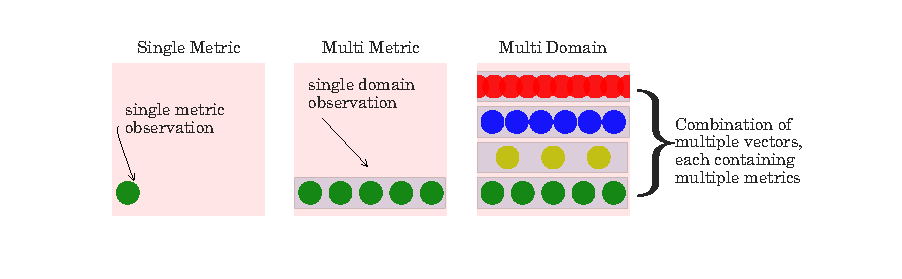
\includegraphics[width=\linewidth]{threat_surface_sum}
	\caption[Multi-Domain Threat Surface]{Multi-Domain Threat Surface}
	\label{fig:threat_surface}
\end{figure}


\section{Autonomous Systems Approach to Trust and Trust Engineering}

\subsection{Autonomous \glspl{manet}}
Autonomy is the capability of an entity to assess its environment and make informed, un-coerced decisions.
In the \gls{manet} context, this sliding scale of capability ranges from basic automated collision avoidance systems while under direct operator control\footnote{For example Automated Driver Assistance Systems entering the consumer vehicle market through the likes of the Tesla P85 and Ford Kuga \cite{Sawade2016}}, through to self-regulating mission guidance and execution, with limited human interaction\footnote{No such systems have been actively deployed, but this form of collaborative autonomy is the centre of much commercial and academic research\cite{Rajesh2015,Autefage2015,Teke2015}}.
This non-deterministic operation presents significant challenges to security and integrity; fundamentally, previously accepted formal verification methodologies for guaranteeing operation are not currently capable of accurately validating the actions and interactions of a fleet or swarm of autonomous nodes in dynamic, noisy environments with imperfect operators\cite{Teke2015}. 
As such an overlapping combination of ``Secure'' and ``Trusted'' approaches are required throughout the lifecycle and operation of an Autonomous \gls{manet} capability to maintain the integrity of such collaborative systems.

\subsection{Trust vs Security vs Integrity}

Early attempts to secure and protect the integrity of \glspl{manet} have relied on various forms of strong-cryptography to protect information being transferred from tampering or malicious inspection.
While such approaches protect the integrity of individual pieces of data, the increased computation, and storage requirements of modern, strong, decentralised cryptographic systems presents a clear avenue for \gls{dos} attacks on \glspl{manet}.
This threat is particularly relevant in resource-constrained networks, where one or more aspects of the environment are limited, be it available power, mobility, data storage, onboard processing, bandwidth, and channel resources such as capacity and delay.
In such networks, where there is a requirement of security and/or integrity monitoring, strong-cryptographic methods present an entirely new opportunity to potential attackers.

One solution to the trade-off between \gls{dos}-protection, and security is the assessment of ``trustworthiness'' of nodes within a local network. 
``Trust'' in this case is an assessment of capability of a node based on previously observed behaviour.
Using this Trust to make simple routing decisions is significantly simpler and faster than strong-cryptographic methods, particularly in multi-hop networks or resource constrained networks\cite{Cordasco2008}.
With Trust being reliant on the runtime awareness of some behaviour, and cryptography on the pre-establishment of some entropy store and the repeated reinforcement of that numerical security, they represent two very different approaches to system integrity with very different costs/benefits and in practice, some elements of both methodologies will be used in different contexts and applications as those applications dictate.

\subsection{Systemic Trust and Trusted Development}
As will be discussed further in \autoref{sec:trust_perspectives}, the ``Trust'' in a system is critical well before a system is activated; the incubation, specification, design, development, production and testing of a system (particularly a system with some \gls{loa} or other non-deterministic operation) is critical to the Trust that an end user can put into that system, and particularly, how much Trust can be exhibited within and between that systems individual components.

\subsection{Trust Operation Against Capable Attackers}\label{sec:capable_attackers}

In any security situation, the hazards and risks of a systemic vulnerability being identified and exploited by an attacker are tightly coupled to the expectation of capability of that attacker.
Within the defence context of this work, it is assumed that any attacking agency has the complexity and resources of a nation state.

This is also one of the primary motivators for this particular direction of work; where increasingly complex and subtle evidentiary security measures (passwords, encryption, etc) are applied, with increasing pressures in computation, connectivity, or communication, the assumption that a slightly-higher-technical-investment will protect a system from state-level espionage or infiltration (or the discovery of some technical flaw in the system) is unfounded, with many examples of cryptographic applications being ``disseminated'' through human or technical failings, but internal and external. 

\section{Maritime Autonomy}

\subsection{title}
\todo{ADD: Intro Section on Marine/AUV inc Pics}

\section{Thesis Layout and Contributions}

\subsection{\fullref{ch:trust_background}}
In this chapter the current literature and research on the concepts, theory, and applications concerning Trust and Trust Management are explored, specifically leaning towards the applications of Trust within Autonomous \glspl{manet}.

In~\autoref{sec:trust_defs}, the abstract quantity of ``trust'' is explored,
In~\autoref{sec:trust_autonomy}, Autonomy and ``Trusted Operation'' of autonomous systems is investigated from a system architects and a system operators perspective.
In~\autoref{sec:trust_manets}, current use and applications of Trusted operation of \glspl{manet} is explored, including current \glspl{tmf}.

\subsection{\fullref{ch:maritime_background}}
In \autoref{ch:maritime_background}, the maritime context is investigated, particularly concerned with the mechanisms of maritime acoustic communications, including the opportunities and challenges of the marine acoustic channel and its modelling(\autoref{sec:marine_comms}).
Additionally, the application scope of \glspl{auv}, littoral and sub-marine operations are explored to provide context to the problem (\autoref{sec:marine_ops}).

\subsection{\fullref{ch:comms_trust}}
In \autoref{ch:comms_trust}, the need for multi-metric trust assessment in \gls{uan} is demonstrated as an example of a harsh network environment.

The operation of a selection of traditional \gls{manet} \glspl{tmf} in this environment is investigated.
These challenges are characterised and results are presented that demonstrate a multi-metric approach to Trust can greatly enhance the effectiveness of \glspl{tmf} in these environments.

In~\autoref{sec:initialsystemcharacterization} an experimental configuration for the marine space is established, and the scenarios and results presented in \citet{Guo11} are reviewed for comparison.
In~\autoref{sec:trustresultsanddiscussion} findings in trust establishment and malicious behaviour detection are presented, comparing with current single metric \glspl{tmf} (Hermes and \gls{otmf}) and the use of this multi-metric (vector) approach to detecting malicious and selfish behaviour in autonomous marine networks is analysed using \gls{mtfm}.

The contributions of this chapter are the first study on the comparative operation and performance of \glspl{tmf} in marine acoustic networks, and a discussion of metric suitability for \glspl{tmf} in marine environments, informing future metric selection for experimenters and theorists, and identifying both the opportunity and need to generate trust from additional domains, such as the physical domain.
Finally, methodology to assess the usefulness of metrics in discriminating against misbehaviours in such constrained, delay-tolerant networks is demonstrated.

Key parts of this chapter were published as \bibentry{Bolster2015}.

\subsubsection{\fullref{ch:physical_trust}}

Current approaches to operational security have been focused on the establishment of trust/security in the communications domain, and ignore other potential threats to the network exploited through physical movement.
This threat is particularly evident in collaborative autonomous systems where nodes are tasked to accomplish some survey / exploration / observation objective in a distributed fashion, where individual nodes make decisions based on the actions of their ``team''. 
This collaboration opens the opportunity for a physically-misbehaving actor to selfishly conserve it's own resources, or maliciously ``drain'' a given target node.
Current security / trust systems applied to \glspl{manet} are not concerned with the threat of such physical misbehaviours.

This chapter proposes a new approach to trust in resource-constrained networks of autonomous systems based on their physical behaviour, using the motion of nodes within a team to detect and potentially identify malicious or failing operation within a cohort.
This is accomplished by looking specifically at operations within the three dimensions of the underwater space, based on kinematics of industry standard \glspl{auv}.
A series of composite metrics based on physical movement are presented and applied to the detection and discrimination of sample physical misbehaviours.
This approach opens the possibility of bringing information about both the physical and communications behaviours of autonomous \glspl{manet} together to strengthen and expand the application of Trust Management Frameworks in sparse and/or resource constrained environments.

Key parts of this chapter were published as \bibentry{Bolster2016}.



\subsubsection{\fullref{ch:multi_domain}}

In this chapter methodology is demonstrated that applies Grey Sequence operations and Grey Generators to provide trust assessment in a sparse, asynchronous metric space across multiple domains of trust.
By utilising information from multiple domains, it is demonstrated that trust assessment can be more accurate and consistent in identifying misbehaviour than in single-domain assessment.
Further, a methodology for assessing the usefulness of individual metrics in this cross-domain space is demonstrated, allowing for the elimination of redundant metrics, simplifying the runtime assessment process.

Key parts of this chapter were published as \bibentry{Bolster2016a}.

\subsubsection{\autoref{ch:conclusion}}

\todo{ADD: Describe Conclusion (Is this redundant?)}




%%%%%%%%%%%%%%%%%%%%%%%%%%%%%%%%%%%%%%%%%%%%%%%%%%%%%%%%%%%%%%%%%%%%%%%%%%%%%%%
